\chapter{Local Search per CSP: Consistenza locale - Local Consistency} \label{ch:Local Search per Crisp CSP: Consistenza locale}
\section{Local Consistency}
\textbf{La consistenza locale} è la condizione che si verifica quando ogni nodo di una rete soddisfa tutti i vincoli che lo coinvolgono. Quest’ultima nei CSP consente di \textbf{ridurre lo spazio di ricerca} di un algoritmo eliminando dal dominio delle variabili i valori che non rispettano i vincoli, cioè che non hanno \textbf{supporto}; può essere definita in rapporto alla consistenza di nodo, arco o cammino.
\begin{itemize}
    \item \textbf{Consistenza di Nodo:} Consiste nella verifica dei valori del dominio di un nodo rispetto ai vincoli del nodo stesso. Ad esempio, se il dominio del nodo $x_1$ è pari a 1,2,3 e il vincolo unario di $x_1$ è $x_1 > 1$, la consistenza di nodo consente di ridurre il dominio di x1 a 2,3 riducendo il processo di ricerca dell’algoritmo.
    \item \textbf{Consistenza di Arco:} Consiste nella verifica dei valori di un dominio di un nodo rispetto ai vincoli binari con un altro nodo. Ad esempio, dati due nodi $x_1$ e $x_2$ con rispettivi domini 1,2,3 e 1,4,5,9, il vincolo $x_2 = x_{1}^2$ consente di ridurre il dominio del nodo x2 a 1,4,9 poichè non sussiste alcun nesso tra il valore 5 dell’insieme dominio di $x_2$ e qualsiasi altro elementi dell’insieme dominio di $x_1$.
    \newpage
    \item \textbf{Consistenza di Cammino:} Consiste nella verifica dei valori di un nodo rispetto ai vincoli n-ari con altri n nodi. La consistenza di cammino è un estenzione della consistenza di arco ed è detta anche k-consistenza. Si distingue dalla consistenza di arco che, invece, è dedicata ai vincoli binari tra due nodi.
\end{itemize}
\subsection{Node Consistency}
In questo caso tutti i vincoli sono unari, le variabili sono rappresentate da dei \textbf{vertici}. Il vertice è \textbf{node consistent} se ogni valore nel dominio delle variabili soddisfa tutti i vincoli unari imposti sulla variabile X. Spesso vengono rappresentati come un cappio o arco che ritorna sullo stesso nodo.
\begin{figure}[htp]
	\centering
    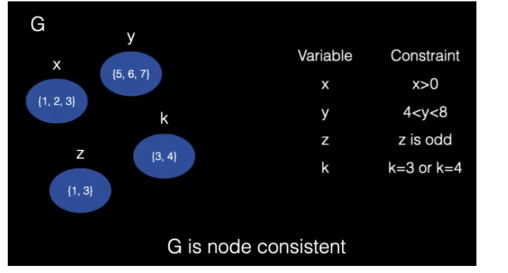
\includegraphics[width=10cm, keepaspectratio]{img/Cap3/node1.png}
    \caption{Esempio grafo node consistent}
\end{figure}
\subsection{Domain Consistency}
L’idea di arc consistency fornisce un metodo veloce di propagazione dei vincoli sostanzialmente più forte del forward checking. Una variabile è consistente al dominio (domain consistent) se nessun valore del dominio del nodo è è dichiarato impossibile da uno qualsiasi dei vincoli. L’idea è di "potare" il più possibile prima di selezionare un valore per le variabili. La domain consistency è stata definita solo per i vincoli che coinvolgono una sola variabile. Quando i vincoli sono binari, possiamo usare gli archi per indicare che un vincolo vale tra una coppia di variabili:
\begin{itemize}
    \item \textbf{un nodo} per ogni variabile
    \item \textbf{un arco} per ogni vincolo
\end{itemize}
\subsection{Arc Consistency}
Quando tutti i vincoli sono binari si parla di arc consistency. Un arco (u,c) è consistente se per ogni valore x del dominio dom(u) esiste un valore y nel dom(v) tale che un assegnamento $u=x$ e $v=y$ soddisfa tutti i vincoli binari che coinvolgono sia u che v.
\subsubsection{Punto fisso e supporto}
Tutto il processo di consistenza locale viene applicato fin quando non si riesce a trovare un punto fisso, cioè fino a quando il dominio delle variabili resta invariato.

\vspace{0.5cm}

\textbf{Problema arc-consistente:} Un problema nel quale applicando local consistency, nessun dominio di nessuna variabile viene modificato.
\\
\textbf{Supporto:} Per la riduzione dobbiamo vedere quali elementi hanno supporto in Y, ovvero quali hanno un assegnamento in Y tale per cui il vincolo viene soddisfatto.
\begin{figure}[htp]
	\centering
    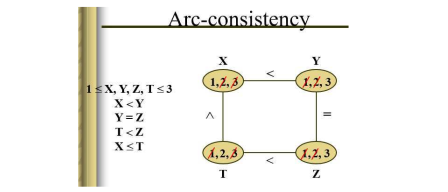
\includegraphics[width=13cm, keepaspectratio]{img/Cap3/esempio-arc.png}
    \caption{Esempio arc-consistency}
\end{figure}
\begin{center}
    Quando $X=1$ esiste un elemento in Y tale per cui $X < Y$? Si, 2,3
    \\Quando $X=2$ esiste un elemento in Y tale per cui $X < Y$? Si, 3
    \\Quando $X=3$ esiste un elemento in Y tale per cui $X < Y$?
    \\No, quindi posso eliminare 3 il dominio di X    
\end{center}
L’operazione che ho fatto si chiama Local Consistency, ma dato che ho utilizzato il vincolo binario si chiama Arc Consistency.
\newpage
\textbf{Conclusione:} In questo caso sono stato molto fortunato perchè ho rimasto 1 solo valore possibile per ogni variabile. Quindi la soluzione è unica e sarà:
\begin{center}
    $X = 1, Y = 3, Z = 3, T = 2$
\end{center}
Se fossi stato meno fortunato comunque avrei ridotto gli elementi del dominio e quindi quando sarei andato a fare la ricerca con backtrack comunque lo spazio di ricerca si sarebbe di molto diminuito (avrei controllano meno assegnamenti)
\vspace{0.3cm}
\\\textbf{Vantaggio rispetto a fare solo Backtracking senza prima applicare local consistency}
\\Se faccio backtrack il dominio degli stati che vado ad esplorare è esponenziale perchè ad X dovrei moltiplicare tutti i possibili valori di Y, a cui dovrei moltiplicare tutti i possibili valori di Z che moltiplico per tutti i valori possibili per T. All’inizio quindi in quel problema si avevano $3^4 = 81$ possibili assegnamenti, mentre se applico prima Local Consistency il problema diventa polinomiale (facile) rispetto al numero di variabili che coinvolgo (in questo caso lo spazio di ricerca mi si riduce ad 1).
\subsection{Algoritmi per Consistenza Locale}
\subsubsection{Procedura Revise}
Per fare diventare un arco (u,v) consistente si cancellano tutti i valori x dal dom(u) che sono incosistenti con tutti i valori in dom(v).
\\Restituisce true se è stata fatta una modifica al dominio di u.
\begin{figure}[htp]
	\centering
    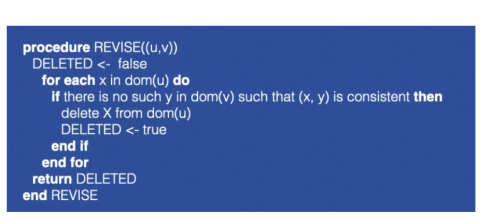
\includegraphics[width=13cm, keepaspectratio]{img/Cap3/revise.png}
    \caption{Procedura REVISE}
\end{figure}
\newpage
\subsubsection{Algoritmo AC-1}
Un singolo passo dell’agoritmo REVISE non è sufficiente. L’algoritmo base per arc consistecy è AC-1, il quale esegue l’algoritmo REVISE finchè il dominio delle variabili cambia. In questo si ripete la procedura REVISE ogni volta che viene modificato un valore in un dominio.
\begin{figure}[htp]
	\centering
    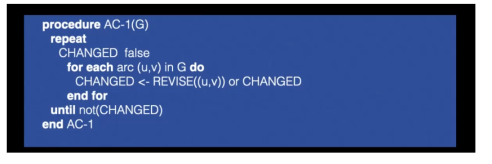
\includegraphics[width=13cm, keepaspectratio]{img/Cap3/ac-1.png}
    \caption{Algoritmo AC-1}
\end{figure}
\\Una sola revisione riuscita di un arco su una particolare iterazione causa la revisione di tutti gli archi nella prossima iterazione anche se gli archi non sono influenzati dal cambiamento.
\\
\textbf{L’inefficienza} sta nel fatto che se anche una singola chiamata alla procedura di REVISE su una particolare iterazione risultasse vera, tutti gli archi verrebbero scansionati nuovamente nella successiva iterazione. Questo però non è sempre necessario, perchè la modifica del dominio di una variabile influenza solamente le variabili che sono collegate a X da un vincolo e non le restanti.
\\La complessità temporale è $O(d^3$ * $n$ * $e)$ e quella spaziale è $O(e$ * $n$ * $d)$.
\newpage
\subsubsection{Algoritmo AC-2}
AC-2 è un algoritmo che può fare arc consistecy in un solo passo attraverso i nodi. Il risultato è ottenuto passando per i nodi in un ordine numerico:
\begin{itemize}
    \item Allegare ad un nodo tutti i valori che non sono in conflitto con i nodi precedentemente assegnati;
    \item Guardando i vicini di questo nodo che sono stati già valutati; se un valore non ha un’assegnazione corrispondente per lo stesso arco, eliminalo;
    \item Ogni volta che qualsiasi valore è cancellato da un arco, guarda ai suoi vicini a sua volta, e si controlla se un loro valore può essere eliminato. Se può essere eliminato, si continua il processo iterativamente finchè non ci sono più cambiamenti che possono essere fatti. Poi si prosegue con gli altri archi.
\end{itemize}
In sostanza si sceglie un ordine fra i nodi, prendiamo ad esempio y come primo e controlliamo tutti i vincoli fra y e k se c’è qualche valore di dom(y) che va in conflitto allora si elimina. Stessa cosa si per l’arco (x,y) se si fa qualche modifica si rimette in coda l’arco in modo da controllare se ci sono altre modifiche da fare. Se un valore b del nodo i è rimosso allora si aggiunge tutti (k,i) alla coda Q, per il controllo degli archi.
\begin{figure}[htp]
	\centering
    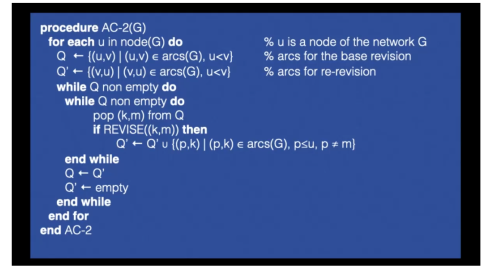
\includegraphics[width=13cm, keepaspectratio]{img/Cap3/ac-2.png}
    \caption{Algoritmo AC-2}
\end{figure}
\\La complessità temporale è $O(d^3$ * $n^2)$ e quella spaziale è $O(n^2$).
\newpage
\subsubsection{Algoritmo AC-3}
AC-3 è un miglioramento di AC-2, alcuni di essi possono essere già essere nella coda Q. Se è così allora non dovrebbero essere inseriti di nuovo.
\begin{figure}[htp]
	\centering
    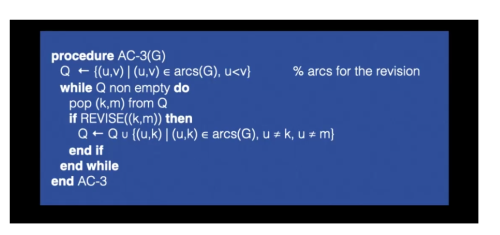
\includegraphics[width=13cm, keepaspectratio]{img/Cap3/ac-3.png}
    \caption{Algoritmo AC-3}
\end{figure}
In sostanza si prende un arco dalla coda Q, si fa la REVISE, se faccio una modifica allora si aggiunge alla coda Q tutti gli archi (u,k) che non sono stati già controllati ovvero $u \neq k$ e $u \neq m$.
\\La complessità temporale è $O(d^2$ * $n^2)$ e quella spaziale è $O(n^2$).
\newpage
\section{Riassunto del prof}
\subsection{Arc-consistency}
Algoritmo che ha la caratteristica di lavorare a livello locale sul CSP. L’obiettivo è quello di semplificarlo in maniera tale da ridurre la quantità di elementi possibili nel dominio e quindi ridurre il tempo necessario quando faccio la ricerca con backtrack.
\\\textbf{Supporto: } un elemento del dominio di X può essere buttato via se non ha supporto in y.
\begin{figure}[htp]
	\centering
    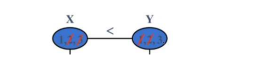
\includegraphics[width=9cm, keepaspectratio]{img/Cap3/riassunto1.png}
\end{figure}
\\Ad esempio, 1 ha supporto in X perchè in Y c’è 2 e 3. Se un elemento non ha supporto lo posso escludere dai valori assegnabili alla variabile. Un problema si dice arc-consistente se ho buttato via tutti gli elementi che NON hanno supporto.

\vspace{0.8cm}

\textbf{Questo è un problema Arc-Consistente?}
\begin{figure}[htp]
	\centering
    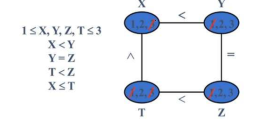
\includegraphics[width=9cm, keepaspectratio]{img/Cap3/riassunto2.png}
\end{figure}
\\No, perchè il 2 andrebbe eliminato da Z. Se riesco a buttare via tutti gli elementi che non hanno supporto allora il problema diventa arc-consistente.
\newpage
\subsection{Soluzione di un CSP}
La soluzione ad un problema è un assegnamento per tutte le variabili.
\\Nel caso in cui fossi interessato solo ad un sottoinsieme di variabili parliamo di \textbf{Vincolo Distinto.}
Le operazioni sono:
\begin{itemize}
    \item  \textbf{Combinazione} tra i vincoli.
    \item \textbf{Proiezione} nel caso in cui esista questo vincolo distinto.
\end{itemize}
Queste operazioni sono di tipo insiemistico nel caso dei CSP classici (Crisp), nel caso in cui invece passiamo a dei problemi di vincoli Soft, e quindi è presente una nozione di priorità tra le soluzioni (il rosso mi costa più del giallo) parliamo di SCSP.
\subsection{Applicare Local Consistency durante il Backtrack}
L’esempio fatto adesso applica la Local Consistency prima di fare Backtrack. Tuttavia è possibile applicarla anche durante la ricerca con backtrack ogni volta che si modifica il dominio di una variabile, vediamo come: (credo che serva solamente sapere che si può fare anche durante e non l’esempio vero e proprio).
\begin{figure}[htp]
	\centering
    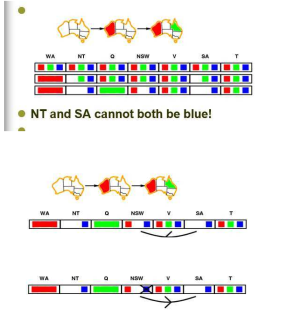
\includegraphics[width=9cm, keepaspectratio]{img/Cap3/riassutno3.png}
\end{figure}
\newpage
\subsubsection{L’Arc Consistency è abbastanza per risolvere il problema?}
Se ci dice bene si, come visto sopra (tolgo talmente tante cose che la soluzione me la trova da solo), ma la maggior parte delle volte permette solamente di restringere lo spazio di ricerca, quindi si può rendere un CSP arc-consistente e poi cercare una soluzione con backtracking; oppure assegnare iterativamente un valore e rendere le variabili restanti arco consistenti. Inoltre, se il dominio
di una variabile diventa vuoto, sappiamo che non esisterà soluzione.
\begin{figure}[htp]
	\centering
    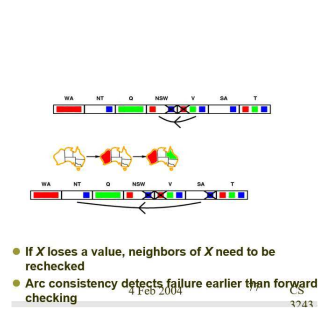
\includegraphics[width=9cm, keepaspectratio]{img/Cap3/riassunto4.png}
\end{figure}
\subsection{Vincolo distinto (Proiezione)}
Alcune volte non ci interessa sapere il valore che possono ottenere tutte le variabili, ma solamente un sottoinsieme di esse. Definiamo quindi il: 
\\
\textbf{Vincolo distinto:} Quali sono gli elementi del problema di cui vogliamo conoscere la soluzione.
\\Sarebbe la proiezione.